\usepackage{cancel}
\usepackage{xcolor}
\usepackage{amsmath}
\usepackage{amssymb}
\usepackage{hyperref}
\usepackage[noblocks]{authblk}
\renewcommand*{\Authsep}{, }
\renewcommand*{\Authand}{, }
\renewcommand*{\Authands}{, }
\renewcommand\Affilfont{\small}
\usepackage[noblocks]{authblk}
\usepackage{tikz}
\usetikzlibrary{calc}
\usetikzlibrary{arrows}
\usetikzlibrary{shapes}
\usetikzlibrary{positioning}
\usetikzlibrary{shapes.geometric}
\usetikzlibrary{decorations}
\renewcommand{\rightarrow}{\tikz[baseline=-0.5ex] \draw[-latex] (0,0) -- (0.5,0);}
\renewcommand{\to}{\rightarrow}
\renewcommand{\leftarrow}{\tikz[baseline=-0.5ex] \draw[latex-] (0,0) -- (0.5,0);}
\newcommand{\rightarrowblue}{\textcolor{blue}{\rightarrow}}
\newcommand{\leftarrowblue}{\textcolor{blue}{\leftarrow}}
\newcommand{\rightarrowred}{\textcolor{red}{\rightarrow}}
\newcommand{\leftarrowred}{\textcolor{red}{\leftarrow}}
\newcommand{\searrowred}{\textcolor{red}{\tikz \draw[-latex] (0,-0) -- (.5,-0.5);}}
\newcommand{\nearrowred}{\textcolor{red}{\tikz \draw[-latex] (0,0) -- (.5,0.5);}}
\newcommand{\rightarrowdotted}{\tikz[baseline=-0.5ex] \draw[dashed, -latex] (0,0) -- (0.5,0);}
\newcommand{\rightarrowdottedred}{\tikz[baseline=-0.5ex] \draw[red, dashed, -latex] (0,0) -- (0.5,0);}
\newcommand{\dottedleftarrowred}{\tikz[baseline=-0.5ex] \draw[red, dashed, latex-] (0,0) -- (0.5,0);}
\newcommand*\circleblue[1]{\tikz[baseline=(char.base)]{\node[shape=circle, draw=blue!100,inner sep=2pt,fill=blue!10, dotted] (char) {#1};}}
\newcommand*\boxedblue[1]{\tikz[baseline=(char.base)]{
\node[shape=rectangle,draw=blue!100,inner sep=2pt,fill=blue!10] (char) {$#1$};}}
\newcommand{\mediation}{A \to \boxed{L} \rightarrowdotted Y}
\newcommand{\commoncause}{
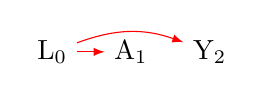
\begin{tikzpicture}
\node [rectangle, draw=white] (L) at (0, 0) {L$_0$};
\node [rectangle, draw=white] (A) at (1, 0) {A$_1$};
\node [rectangle, draw=white] (Y) at (2, 0) {Y$_2$};
\draw [-latex, draw = red] (L) to (A);
\draw [-latex, draw = white, dotted] (A) to (Y);
\draw [-latex, bend left=20, draw=red] (L) to (Y);
\end{tikzpicture}
}
\newcommand{\commoncausesolved}{
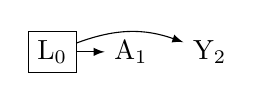
\begin{tikzpicture}
\node [rectangle, draw=black] (L) at (0, 0) {L$_0$};
\node [rectangle, draw=white] (A) at (1, 0) {A$_1$};
\node [rectangle, draw=white] (Y) at (2, 0) {Y$_2$};
\draw [-latex, draw = black] (L) to (A);
\draw [-latex, draw = white, dotted] (A) to (Y);
\draw [-latex, bend left=20, draw=black] (L) to (Y);
\end{tikzpicture}
}
\newcommand{\commoncausesolvedchild}{
 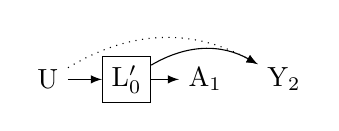
\begin{tikzpicture}
 \node [rectangle, draw=white] (L) at (-1, 0) {U};
 \node [rectangle, draw=black] (L1) at (0, 0) {L$^{\prime}_0$};
 \node [rectangle, draw=white] (A) at (1, 0) {A$_1$};
 \node [rectangle, draw=white] (Y) at (2, 0) {Y$_2$};                        
 \draw [-latex, draw = black] (L) to (L1);
 \draw [-latex, draw = black] (L1) to (A);
 \draw [-latex, draw = black, bend left = 30, dotted] (L) to (Y);
 \draw [-latex, bend left=30, draw=black] (L1) to (Y);
 \end{tikzpicture}
 }
 \newcommand{\child}{
 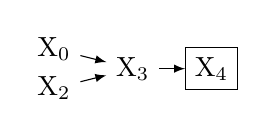
\begin{tikzpicture}
 \node [rectangle, draw=white] (A) at (0, .25) {X$_0$};
 \node [rectangle, draw=white] (L) at (1, 0) {X$_3$};
 \node [rectangle, draw=black] (L1) at (2, 0) {X$_4$};
 \node [rectangle, draw=white] (Y) at (0, -.25) {X$_2$};
 \draw [-latex, draw = black] (A) -- (L);
 \draw [-latex, draw = black] (Y) -- (L);
 \draw [-latex, draw = black] (L) -- (L1);
 \end{tikzpicture}
 }
 \newcommand{\descendant}{
 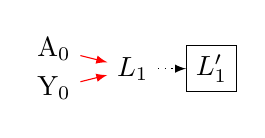
\begin{tikzpicture}
 \node [rectangle, draw=white] (A) at (0, .25) {A$_0$};
 \node [rectangle, draw=white] (L) at (1, 0) {$L_1$};
 \node [rectangle, draw=black] (L1) at (2, 0) {$L'_1$};
 \node [rectangle, draw=white] (Y) at (0, -.25) {Y$_0$};
 \draw [-latex, draw = red] (A) -- (L);
 \draw [-latex, draw = red] (Y) -- (L);
 \draw [-latex, draw = black,dotted] (L) -- (L1);
 \end{tikzpicture}
 }
 \newcommand{\collider}{
 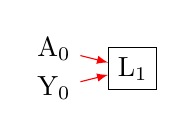
\begin{tikzpicture}
 \node [rectangle, draw=white] (A) at (0, .25) {A$_0$};
 \node [rectangle, draw=black] (L) at (1, 0) {L$_1$};
 \node [rectangle, draw=white] (Y) at (0, -.25) {Y$_0$};
 \draw [-latex, draw = red] (A) to (L);
 \draw [-latex, draw = red] (Y) to (L);
 \end{tikzpicture}
 }
 \newcommand{\mediator}{
 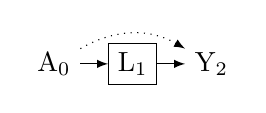
\begin{tikzpicture}
 \node [rectangle, draw=white] (A) at (0, 0) {A$_0$};
 \node [rectangle, draw=black] (L) at (1, 0) {L$_1$};
 \node [rectangle, draw=white] (Y) at (2, 0) {Y$_2$};
 \draw [-latex, draw = black] (A) to (L);
 \draw [-latex, draw = black] (L) to (Y);
 \draw [-latex,  bend left=30, draw=black, dotted] (A) to (Y);
 \end{tikzpicture}
 }
 \newcommand{\mediatorm}{
 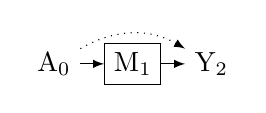
\begin{tikzpicture}
 \node [rectangle, draw=white] (A) at (0, 0) {A$_0$};
 \node [rectangle, draw=black] (M) at (1, 0) {M$_1$};
 \node [rectangle, draw=white] (Y) at (2, 0) {Y$_2$};
 \draw [-latex, draw = black] (A) to (M);
 \draw [-latex, draw = black] (M) to (Y);
 \draw [-latex,  bend left=30, draw=black, dotted] (A) to (Y);
 \end{tikzpicture}
 }
 \newcommand{\chain}{
 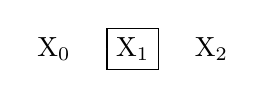
\begin{tikzpicture}
 \node [rectangle, draw=white] (A) at (0, 0) {X$_0$};
 \node [rectangle, draw=black] (M) at (1, 0) {X$_1$};
 \node [rectangle, draw=white] (Y) at (2, 0) {X$_2$};
 \draw [-latex, draw = white] (A) to (M);
 \draw [-latex, draw = white] (M) to (Y);
 \end{tikzpicture}
 }
 \renewcommand*{\chain}{
 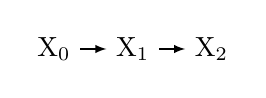
\begin{tikzpicture}
 \node [rectangle, draw=white] (A) at (0, 0) {X$_0$};
 \node [rectangle, draw=white] (M) at (1, 0) {X$_1$};
 \node [rectangle, draw=white] (Y) at (2, 0) {X$_2$};
 \draw [-latex, draw = black] (A) to (M);
 \draw [-latex, draw = black] (M) to (Y);
 \end{tikzpicture}
 }
 \newcommand{\immorality}{
 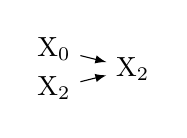
\begin{tikzpicture}
 \node [rectangle, draw=white] (A) at (0, .25) {X$_0$};
 \node [rectangle, draw=white] (L) at (1, 0) {X$_2$};
 \node [rectangle, draw=white] (Y) at (0, -.25) {X$_2$};
 \draw [-latex, draw = black] (A) to (L);
 \draw [-latex, draw = black] (Y) to (L);
 \end{tikzpicture}
 }
 \newcommand{\fork}{
 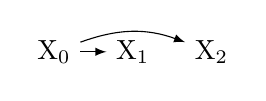
\begin{tikzpicture}
 \node [rectangle, draw=white] (L) at (0, 0) {X$_0$};
 \node [rectangle, draw=white] (A) at (1, 0) {X$_1$};
 \node [rectangle, draw=white] (Y) at (2, 0) {X$_2$};
 \draw [-latex, draw = black] (L) to (A);
 \draw [-latex, draw = white, dotted] (A) to (Y);
 \draw [-latex, bend left=20, draw=black] (L) to (Y);
 \end{tikzpicture}
 }
\newcommand{\mbias}{
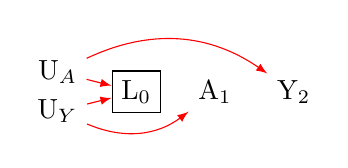
\begin{tikzpicture}
\node [rectangle, draw=white] (UA) at (0, .25) {U$_A$};
\node [rectangle, draw=white] (UY) at (0, -.25) {U$_Y$};
\node [rectangle, draw=black] (L) at (1, 0) {L$_0$};
\node [rectangle, draw=white] (A) at (2, 0) {A$_1$};
\node [rectangle, draw=white] (Y) at (3, 0) {Y$_2$};
\draw [-latex, draw = red] (UA) to (L);
\draw [-latex, draw = red] (UY) to (L);
\draw [-latex, draw = red, bend left = 30] (UA) to (Y);
\draw [-latex, draw = red, bend right = 30] (UY) to (A);
\end{tikzpicture}
}
\newcommand{\mbiasdoomed}{
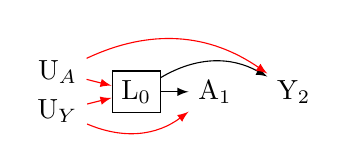
\begin{tikzpicture}
\node [rectangle, draw=white] (UA) at (0, .25) {U$_A$};
\node [rectangle, draw=white] (UY) at (0, -.25) {U$_Y$};
\node [rectangle, draw=black] (L) at (1, 0) {L$_0$};
\node [rectangle, draw=white] (A) at (2, 0) {A$_1$};
\node [rectangle, draw=white] (Y) at (3, 0) {Y$_2$};
\draw [-latex, draw = red] (UA) to (L);
\draw [-latex, draw = red] (UY) to (L);
\draw [-latex, draw = black, bend left = 30] (L) to (Y);
\draw [-latex, draw = black] (L) to (A);
\draw [-latex, draw = red, bend left = 30] (UA) to (Y);
\draw [-latex, draw = red, bend right = 30] (UY) to (A);
\end{tikzpicture}
}
\newcommand{\mbiassolved}{
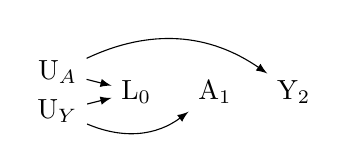
\begin{tikzpicture}
\node [rectangle, draw=white] (UA) at (0, .25) {U$_A$};
\node [rectangle, draw=white] (UY) at (0, -.25) {U$_Y$};
\node [rectangle, draw=white] (L) at (1, 0) {L$_0$};
\node [rectangle, draw=white] (A) at (2, 0) {A$_1$};
\node [rectangle, draw=white] (Y) at (3, 0) {Y$_2$};
\draw [-latex, draw = black] (UA) to (L);
\draw [-latex, draw = black] (UY) to (L);
\draw [-latex, draw = black, bend left = 30] (UA) to (Y);
\draw [-latex, draw = black, bend right = 30] (UY) to (A);
\end{tikzpicture}
}
\newcommand{\measurementerroruncorrelated}{
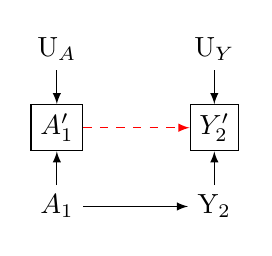
\begin{tikzpicture}
\node [rectangle, draw=white] (UA) at (0, 1) {U$_A$};
\node [rectangle, draw=white] (A) at (0, -1) {$A_1$};
\node [rectangle, draw=black] (A1) at (0, 0) {$A'_1$};
\node [rectangle, draw=white] (UY) at (2, 1) {U$_Y$};
\node [rectangle, draw=black] (Y1) at (2, 0) {$Y'_2$};
\node [rectangle, draw=white] (Y) at (2, -1) {Y$_2$};
\draw [-latex, draw = black] (UA) to (A1);
\draw [-latex, draw = black] (A) to (A1);
\draw [-latex, draw = black] (UY) to (Y1);
\draw [-latex, draw = black] (Y) to (Y1);
\draw [-latex, draw = black] (A) to (Y);
\draw [-latex, draw = red, dashed] (A1) to (Y1);
\end{tikzpicture}
}
\newcommand{\measurementerrorcorrelated}{
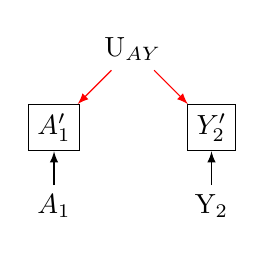
\begin{tikzpicture}
\node [rectangle, draw=white] (U) at (1, 1) {U$_{AY}$};
\node [rectangle, draw=white] (A) at (0, -1) {$A_1$};
\node [rectangle, draw=black] (A1) at (0, 0) {$A'_1$};
\node [rectangle, draw=black] (Y1) at (2, 0) {$Y'_2$};
\node [rectangle, draw=white] (Y) at (2, -1) {Y$_2$};
\draw [-latex, draw = red] (U) to (A1);
\draw [-latex, draw = black] (A) to (A1);
\draw [-latex, draw = red] (U) to (Y1);
\draw [-latex, draw = black] (Y) to (Y1);
\end{tikzpicture}
}
\newcommand{\measurementerrordirected}{
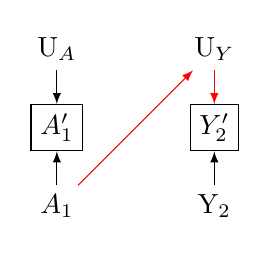
\begin{tikzpicture}
\node [rectangle, draw=white] (UA) at (0, 1) {U$_A$};
\node [rectangle, draw=white] (A) at (0, -1) {$A_1$};
\node [rectangle, draw=black] (A1) at (0, 0) {$A'_1$};
\node [rectangle, draw=white] (UY) at (2, 1) {U$_Y$};
\node [rectangle, draw=black] (Y1) at (2, 0) {$Y'_2$};
\node [rectangle, draw=white] (Y) at (2, -1) {Y$_2$};
\draw [-latex, draw = black] (UA) to (A1);
\draw [-latex, draw = black] (A) to (A1);
\draw [-latex, draw = red] (UY) to (Y1);
\draw [-latex, draw = black] (Y) to (Y1);
\draw [-latex, draw = red] (A) to (UY);
\end{tikzpicture}
}
\newcommand{\measurementerrorcorrelateddirected}{
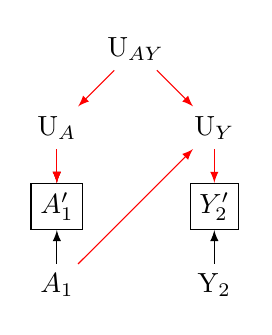
\begin{tikzpicture}
\node [rectangle, draw=white] (UAY) at (1, 2) {U$_{AY}$};
\node [rectangle, draw=white] (UA) at (0, 1) {U$_A$};
\node [rectangle, draw=white] (A) at (0, -1) {$A_1$};
\node [rectangle, draw=black] (A1) at (0, 0) {$A'_1$};
\node [rectangle, draw=white] (UY) at (2, 1) {U$_Y$};
\node [rectangle, draw=black] (Y1) at (2, 0) {$Y'_2$};
\node [rectangle, draw=white] (Y) at (2, -1) {Y$_2$};
\draw [-latex, draw = black] (UA) to (A1);
\draw [-latex, draw = black] (A) to (A1);
\draw [-latex, draw = red] (UY) to (Y1);
\draw [-latex, draw = black] (Y) to (Y1);
\draw [-latex, draw = red] (A) to (UY);
\draw [-latex, draw = red] (UA) to (A1);
\draw [-latex, draw = red] (UA) to (A1);
\draw [-latex, draw = red] (UA) to (A1);
\draw [-latex, draw = red] (UAY) to (UA);
\draw [-latex, draw = red] (UAY) to (UY);
\end{tikzpicture}
}
\newcommand{\measurementerrorcorrelateddirectedy}{
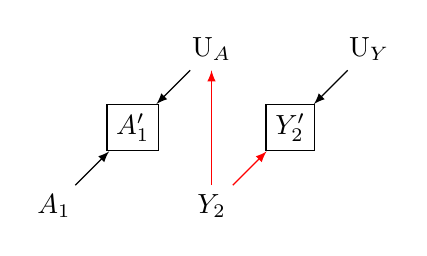
\begin{tikzpicture}
\node [rectangle, draw=white] (A) at (0, -1) {$A_1$};
\node [rectangle, draw=white] (Y) at (2, -1) {$Y_2$};
\node [rectangle, draw=white] (UA) at (2, 1) {U$_A$};
\node [rectangle, draw=black] (A1) at (1, 0) {$A'_1$};
\node [rectangle, draw=white] (UY) at (4, 1) {U$_Y$};
\node [rectangle, draw=black] (Y1) at (3, 0) {$Y'_2$};
\draw [-latex, draw = black] (UA) to (A1);
\draw [-latex, draw = black] (A) to (A1);
\draw [-latex, draw = black] (UY) to (Y1);
\draw [-latex, draw = red] (Y) to (Y1);
\draw [-latex, draw = red] (Y) to (UA);
\end{tikzpicture}
}
\newcommand{\twonodesconnected}{
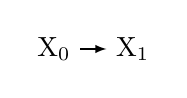
\begin{tikzpicture}
\node [rectangle, draw=white] (A) at (0, 0) {X$_0$};
\node [rectangle, draw=white] (Y) at (1, 0) {X$_1$};
\draw [-latex, draw = black] (A) to (Y);
\end{tikzpicture}
}
\newcommand{\twonodesseparated}{
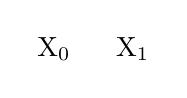
\begin{tikzpicture}
\node [rectangle, draw=white] (A) at (0, 0) {X$_0$};
\node [rectangle, draw=white] (Y) at (1, 0) {X$_1$};
\draw [-latex, draw = white] (A) to (Y);
\end{tikzpicture}
}
\newcommand{\ayseparated}{
\begin{tikzpicture}
\node [rectangle, draw=white] (A) at (0, 0) {A$_1$};
\node [rectangle, draw=white] (Y) at (1.5, 0) {Y$_2$};
\draw [-latex, draw = white] (A) to (Y);
\end{tikzpicture}
}
\newcommand{\ayconnected}{
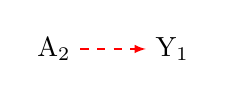
\begin{tikzpicture}
\node [rectangle, draw=white] (A) at (0, 0) {A$_2$};
\node [rectangle, draw=white] (Y) at (1.5, 0) {Y$_1$};
\draw [-latex, draw = red, dashed] (A) to (Y);
\end{tikzpicture}
}
\newcommand{\restrictionbig}{
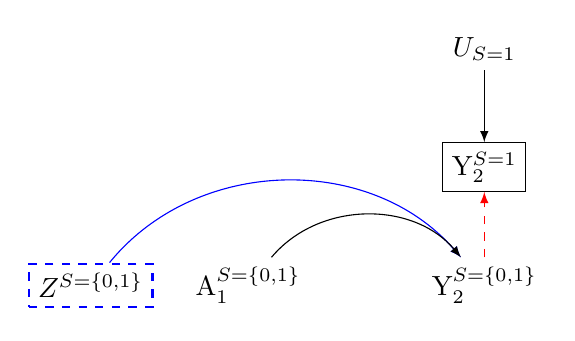
\begin{tikzpicture}
\node [rectangle, draw=white] (A) at (0, 0) {A$_1^{S=\{0,1\}}$};
\node [rectangle, thick, dashed, draw=blue] (Z) at (-2, 0) {$Z^{S=\{0,1\}}$};
\node [rectangle, draw=black, fill=red!0](YS) at (3, 1.5) {Y$_2^{S=1}$};
\node [rectangle, draw=white,text=black] (Y) at (3,0) {Y$_2^{S=\{0,1\}}$};
\node [rectangle, draw=white,text=black] (U) at (3,3) {$U_{S=1}$};
\draw [-latex, draw = red, dashed] (Y) to (YS);
\draw [-latex, bend left=50, draw=blue] (Z) to (Y);
\draw [-latex, draw=black, bend left =50] (A) to (Y);
\draw [-latex, draw=black] (U) to (YS);
\end{tikzpicture}
}
\renewcommand*{\restriction}{
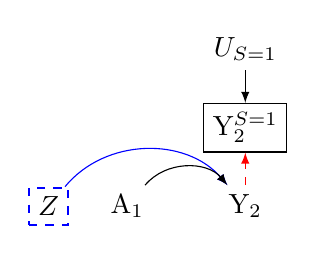
\begin{tikzpicture}
\node [rectangle, draw=white] (A) at (0, 0) {A$_1$};
\node [rectangle, thick, dashed, draw=blue] (Z) at (-1, 0) {$Z$};
\node [rectangle, draw=black, fill=red!0](YS) at (1.5, 1) {Y$_2^{S=1}$};
\node [rectangle, draw=white,text=black] (Y) at (1.5,0) {Y$_2$};
\node [rectangle, draw=white,text=black] (U) at (1.5,2) {$U_{S=1}$};
\draw [-latex, dashed, draw = red] (Y) to (YS);
\draw [-latex, bend left=50, draw=blue] (Z) to (Y);
\draw [-latex, draw=black, bend left =50] (A) to (Y);
\draw [-latex, draw=black] (U) to (YS);
\end{tikzpicture}
}
\newcommand{\restrictioncore}{
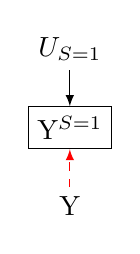
\begin{tikzpicture}
\node [rectangle, draw=black, fill=red!0](YS) at (0, 1) {Y$^{S=1}$};
\node [rectangle, draw=white,text=black] (Y) at (0,0) {Y};
\node [rectangle, draw=white,text=black] (U) at (0,2) {$U_{S=1}$};
\draw [-latex, draw = red, dashed] (Y) to (YS);
\draw [-latex, draw=black] (U) to (YS);
\end{tikzpicture}
}
\newcommand{\indirecteffectmodification}{
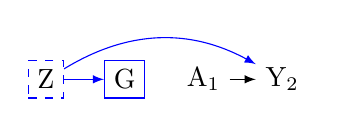
\begin{tikzpicture}
\node [rectangle, draw=white] (A) at (0, 0) {A$_{1}$};
\node [rectangle, draw=white] (Y) at (1, 0) {Y$_{2}$};
\node [rectangle,dashed,draw=blue] (Z) at (-2,0) {Z};
\node [rectangle, draw=blue] (G) at (-1, 0) {G};
\draw [-latex, draw=black] (A) to (Y);
\draw [-latex, bend left, draw=blue] (Z) to (Y);
\draw [-latex, draw = blue] (Z) to (G);
\end{tikzpicture}
}
\newcommand{\directeffectmodification}{
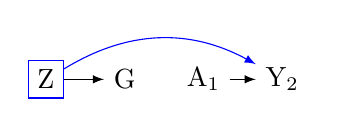
\begin{tikzpicture}
\node [rectangle, draw=white] (A) at (0, 0) {A$_{1}$};
\node [rectangle, draw=white] (Y) at (1, 0) {Y$_{2}$};
\node [rectangle, draw=blue] (Z) at (-2,0) {Z};
\node [rectangle, draw=white] (G) at (-1, 0) {G};
\draw [-latex, draw=black] (A) to (Y);
\draw [-latex, bend left, draw=blue] (Z) to (Y);
\draw [-latex, draw = black] (Z) to (G);
\end{tikzpicture}
}
\newcommand{\collidereffectmodification}{
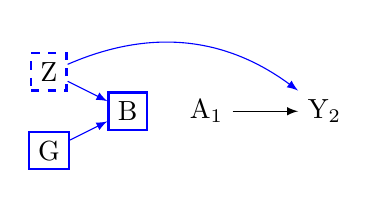
\begin{tikzpicture}
\node [rectangle, draw=white] (A) at (0, 0) {A$_{1}$};
\node [rectangle, draw=white] (Y) at (1.5, 0) {Y$_{2}$};
\node [rectangle, dashed, thick, draw=blue] (Z) at (-2, .5) {Z};
\node [rectangle, thick, draw=blue] (G) at (-2, -.5) {G};
\node [rectangle, thick, draw=blue] (B) at (-1,0) {B};
\draw [-latex, draw=black] (A) to (Y);
\draw [-latex, bend left, draw=blue] (Z) to (Y);
\draw [-latex, draw=blue] (Z) to (B);
\draw [-latex, draw=blue] (G) to (B);
\end{tikzpicture}
}
\newcommand{\childeffectmodification}{
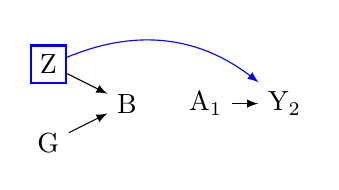
\begin{tikzpicture}
\node [rectangle, draw=white] (A) at (0, 0) {A$_{1}$};
\node [rectangle, draw=white] (Y) at (1, 0) {Y$_{2}$};
\node [rectangle, thick, draw=blue] (Z) at (-2, .5) {Z};
\node [rectangle, draw=white] (G) at (-2, -.5) {G};
\node [rectangle, draw=white] (B) at (-1,0) {B};
\draw [-latex, draw=black] (A) to (Y);
\draw [-latex, bend left, draw=blue] (Z) to (Y);
\draw [-latex, draw=black] (Z) to (B);
\draw [-latex, draw=black] (G) to (B);
\end{tikzpicture}
}
\newcommand{\effectmodification}{
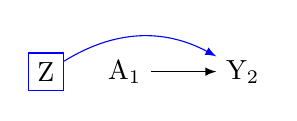
\begin{tikzpicture}
\node [rectangle, draw=white] (A) at (0, 0) {A$_{1}$};
\node [rectangle, draw=white] (Y) at (1.5, 0) {Y$_{2}$};
\node [rectangle,draw=blue] (Z) at (-1,0) {Z};
\draw [-latex, draw=black] (A) to (Y);
\draw [-latex, bend left, draw=blue] (Z) to (Y);
\end{tikzpicture}
}
\newcommand{\effectmodificationunconditioned}{
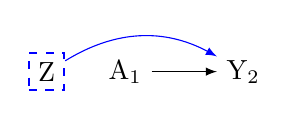
\begin{tikzpicture}
\node [rectangle, draw=white] (A) at (0, 0) {A$_{1}$};
\node [rectangle, draw=white] (Y) at (1.5, 0) {Y$_{2}$};
\node [rectangle, dashed, thick, draw=blue] (Z) at (-1,0) {Z};
\draw [-latex, draw=black] (A) to (Y);
\draw [-latex, bend left, draw=blue] (Z) to (Y);
\end{tikzpicture}
}